% imports
\begin{figure*}
\centering
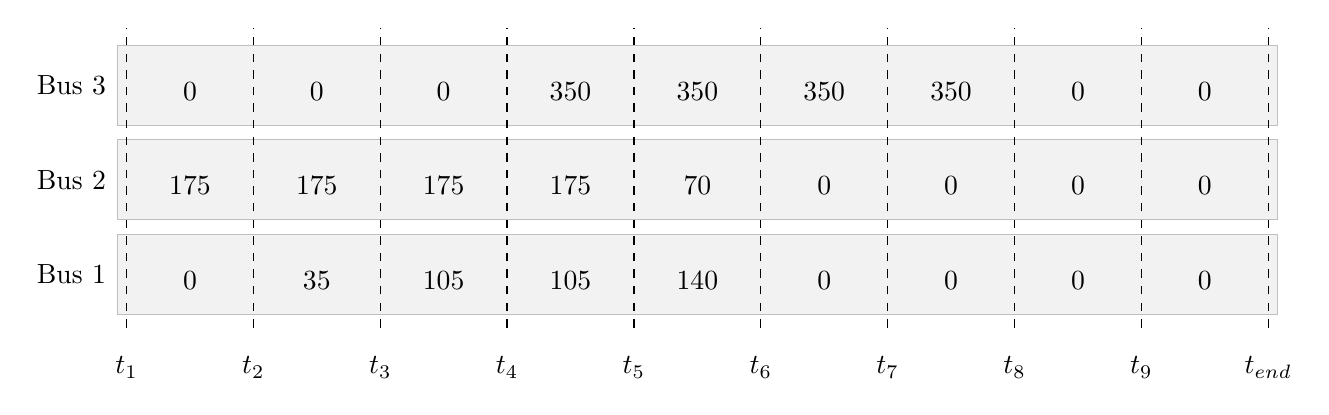
\begin{tikzpicture}
	\node[rectangle, draw=gray!50, fill=gray!10, minimum width=5.8in, minimum height=0.4in](bus1Box) at (7.75,0.8){};
	\node(bus1BoxLabel) at (-0.2, 0.8){Bus 1}; 
	
	\node[rectangle, draw=gray!50, fill=gray!10, minimum width=5.8in, minimum height=0.4in](bus2Box) at (7.75,2){};
	\node(bus1BoxLabel) at (-0.2, 2.0){Bus 2};
	
	\node[rectangle, draw=gray!50, fill=gray!10, minimum width=5.8in, minimum height=0.4in](bus3Box) at (7.75,3.2){};
	\node(bus1BoxLabel) at (-0.2, 3.2){Bus 3};
	
	\foreach \curLab/\preLab[count=\c, evaluate=\c as \pos using {0.5 + (\c - 1)*14.5/9}] in {t_1/t_1, t_2/t_1, t_3/t_2, t_4/t_3, t_5/t_4, t_6/t_7, t_7/t_6, t_8/t_7, t_9/t_8, t_{end}/t_9}
	{
		\node[label=below:$\curLab$](b\c) at (\pos, 0){};
		\node(t) at (\pos, 3.8){};
		\draw[dashed, line width=0.5pt] (b\c.north) -- (t.north); 
		\ifnum\c>1 
			\node(b1Curr) at (\pos, 0.8 - 0.2){};
			\node(b2Curr) at (\pos, 2.0 - 0.2){};
			\node(b3Curr) at (\pos, 3.2 - 0.2){};
			\path(b1Prev.east) -- node(node1\c)[midway, above]{}(b1Curr.west);
			\path(b2Prev.east) -- node(node2\c)[midway, above]{}(b2Curr.west);
			\path(b3Prev.east) -- node(node3\c)[midway, above]{}(b3Curr.west);	
		\fi
			\node(b1Prev) at (\pos, 0.8 - 0.2){};
			\node(b2Prev) at (\pos, 2.0 - 0.2){};
			\node(b3Prev) at (\pos, 3.2 - 0.2){};	
	}
	\path (b9.south) -- node[midway, below=0.1in]{$\hdots$}(b10.south);
	\node at (node12.center){0};
	\node at (node13.center){35};
	\node at (node14.center){105};
	\node at (node15.center){105};
	\node at (node16.center){140};
	\node at (node17.center){0};
	\node at (node18.center){0};
	\node at (node19.center){0};
	\node at (node110.center){0};
	\node at (node22.center){175};
	\node at (node23.center){175};
	\node at (node24.center){175};
	\node at (node25.center){175};
	\node at (node26.center){70};
	\node at (node27.center){0};
	\node at (node28.center){0};
	\node at (node29.center){0};
	\node at (node210.center){0};
	\node at (node32.center){0};
	\node at (node33.center){0};
	\node at (node34.center){0};
	\node at (node35.center){350};
	\node at (node36.center){350};
	\node at (node37.center){350};
	\node at (node38.center){350};
	\node at (node39.center){0};
	\node at (node310.center){0};

\end{tikzpicture}
\caption{An example solution to a 3-bus, 2-charger scenario from $p_4$}
\label{fig:solutionExample}
\end{figure*}

\begin{figure*}
\centering
\scalebox{0.8}{
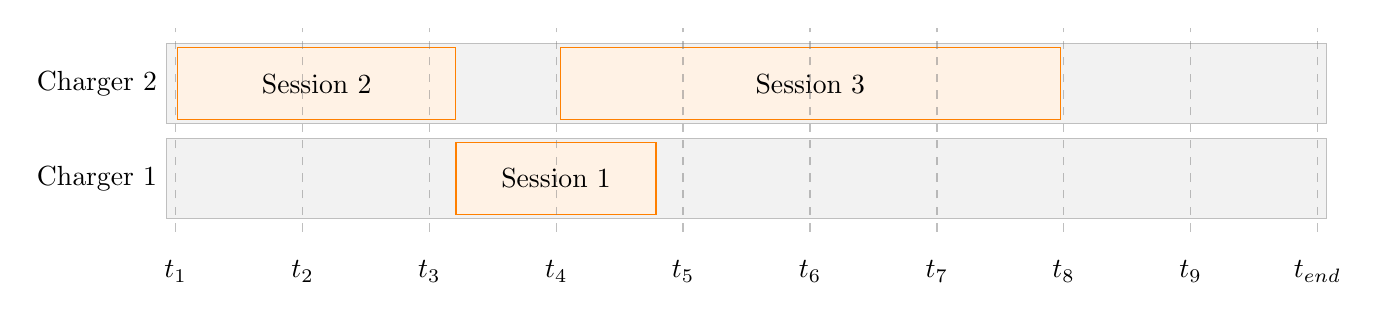
\begin{tikzpicture}
	\node[rectangle, draw=gray!50, fill=gray!10, minimum width=5.8in, minimum height=0.4in](bus1Box) at (7.75,0.8){};
	\node(bus1BoxLabel) at (-0.5, 0.8){Charger 1}; 

	\node[rectangle, draw=gray!50, fill=gray!10, minimum width=5.8in, minimum height=0.4in](bus2Box) at (7.75,2){};
	\node(bus1BoxLabel) at (-0.5, 2.0){Charger 2};
	\node[rectangle, draw=orange!100, fill=orange!10, minimum width=1.3915in, minimum height=0.36in](charge111) at (2.29, 2){Session 2}; 
	\node[rectangle, draw=orange!100, fill=orange!10, minimum width=1in, minimum height=0.36in](charge111) at (5.33, 0.8){Session 1};
	\node[rectangle, draw=orange!100, fill=orange!10, minimum width=2.50in, minimum height=0.36in](charge111) at (8.56, 2){Session 3};


	\foreach \curLab/\preLab[count=\c, evaluate=\c as \pos using {0.5 + (\c - 1)*14.5/9}] in {t_1/t_1, t_2/t_1, t_3/t_2, t_4/t_3, t_5/t_4, t_6/t_7, t_7/t_6, t_8/t_7, t_9/t_8, t_{end}/t_9}
		{
			\node[label=below:$\curLab$](b\c) at (\pos, 0){};
			\node(t) at (\pos, 2.58){};
			\draw[dashed, line width=0.5pt, black!50, opacity=0.5] (b\c.north) -- (t.north); 
		}
		\path (b9.south) -- node[midway, below=0.1in]{$\hdots$}(b10.south); 
\end{tikzpicture}}
\caption{Demonstrates the solution to $p_5$}
\label{fig:secondSolutionExample}
\end{figure*}



\begin{figure*}
\centering
\scalebox{0.8}{
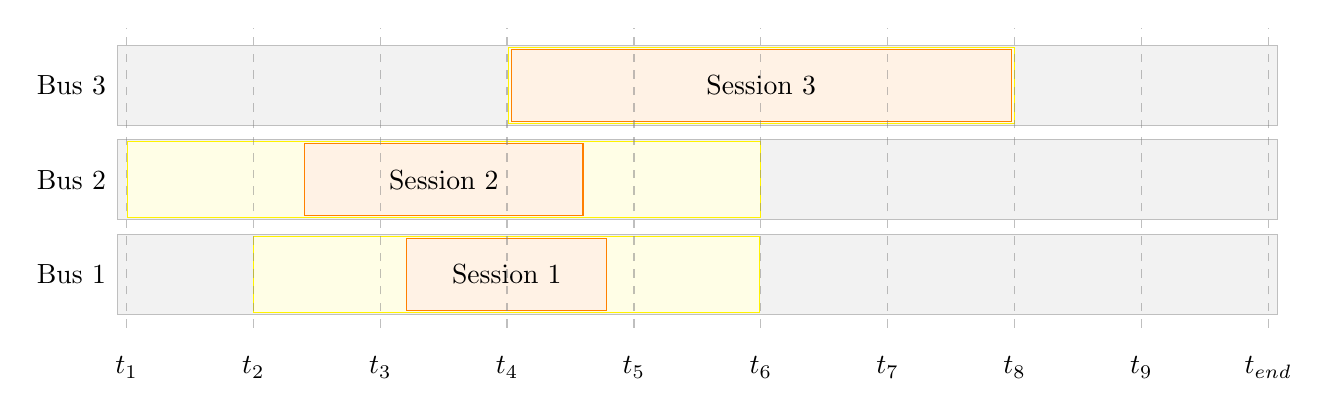
\begin{tikzpicture}
	\node[rectangle, draw=gray!50, fill=gray!10, minimum width=5.8in, minimum height=0.4in](bus1Box) at (7.75,0.8){};
	\node(bus1BoxLabel) at (-0.2, 0.8){Bus 1}; 
	\node[rectangle, draw=yellow!100, fill=yellow!10, minimum width=2.53in, minimum height=0.38in](charge11) at (5.33, 0.8){};
	\node[rectangle, draw=orange!100, fill=orange!10, minimum width=1in, minimum height=0.36in](charge111) at (5.33, 0.8){Session 1};

	\node[rectangle, draw=gray!50, fill=gray!10, minimum width=5.8in, minimum height=0.4in](bus2Box) at (7.75,2){};
	\node(bus1BoxLabel) at (-0.2, 2.0){Bus 2};
	\node[rectangle, draw=yellow!100, fill=yellow!10, minimum width=3.1625in, minimum height=0.38in](charge11) at (4.53, 2){};
	\node[rectangle, draw=orange!100, fill=orange!10, minimum width=1.3915in, minimum height=0.36in](charge111) at (4.53, 2){Session 2};
	
	\node[rectangle, draw=gray!50, fill=gray!10, minimum width=5.8in, minimum height=0.4in](bus3Box) at (7.75,3.2){};
	\node(bus1BoxLabel) at (-0.2, 3.2){Bus 3}; 
	\node[rectangle, draw=yellow!100, fill=yellow!10, minimum width=2.53in, minimum height=0.38in](charge11) at (8.56, 3.2){};
	\node[rectangle, draw=orange!100, fill=orange!10, minimum width=2.50in, minimum height=0.36in](charge111) at (8.56, 3.2){Session 3};


	\foreach \curLab/\preLab[count=\c, evaluate=\c as \pos using {0.5 + (\c - 1)*14.5/9}] in {t_1/t_1, t_2/t_1, t_3/t_2, t_4/t_3, t_5/t_4, t_6/t_7, t_7/t_6, t_8/t_7, t_9/t_8, t_{end}/t_9}
		{
			\node[label=below:$\curLab$](b\c) at (\pos, 0){};
			\node(t) at (\pos, 3.8){};
			\draw[dashed, line width=0.5pt, black!50, opacity=0.5] (b\c.north) -- (t.north); 
		}
		\path (b9.south) -- node[midway, below=0.1in]{$\hdots$}(b10.south); 
\end{tikzpicture}}
\caption{Demonstrates how results from $p_4$ can be reexpressed in terms of continuous variables} 
\label{fig:refactorExample}
\end{figure*}



\begin{figure*}
\centering
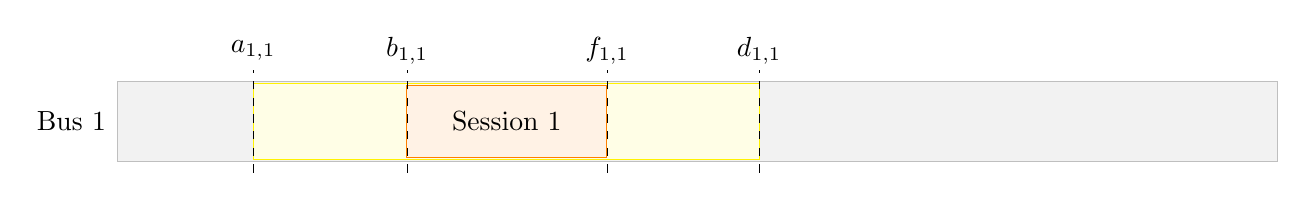
\begin{tikzpicture}
	\node[rectangle, draw=gray!50, fill=gray!10, minimum width=5.8in, minimum height=0.4in](bus1Box) at (7.75,0.8){};
	\node(bus1BoxLabel) at (-0.2, 0.8){Bus 1}; 
	\node[rectangle, draw=yellow!100, fill=yellow!10, minimum width=2.53in, minimum height=0.38in](charge11) at (5.33, 0.8){};
	\node[rectangle, draw=orange!100, fill=orange!10, minimum width=1in, minimum height=0.36in](charge111) at (5.33, 0.8){Session 1}; 
	\draw[dashed] (0.83in,0.15) -- (0.83in,1.45);
	\node at (0.83in,1.7){$a_{1,1}$};
	\draw[dashed] (3.36in, 0.15) -- (3.36in, 1.45);
	\node at (3.36in,1.7){$d_{1,1}$};
	\draw[dashed] (1.6in, 0.15) -- (1.6in, 1.45);
	\node at (1.6in,1.7){$b_{1,1}$};
	\draw[dashed] (2.6in, 0.15) -- (2.6in, 1.45);
	\node at (2.6in,1.7){$f_{1,1}$};
\end{tikzpicture}
\caption{Gives variables of optimization for $p_5$}
\label{fig:secondProgramVars}
\end{figure*} 


\section{Charge Schedules}
The results from the Linear Program defined in the previous section give us a general estimate of how much and when buses should charge, however we must still address two primary issues. The first is defining concrete start and stop times for each charge session. The second is limiting the charge sessions to a finite number of chargers. After solving the first program, we take the results and derive {\it preliminary} intervals and average power consumptions for each charge session.  
\par For example, consider a solution to a three bus, two charger scenario given in Fig. \ref{fig:solutionExample}.
Note that there appears to be three buses charging at the same time from $t_5$ to $t_6$ even though there are only two chargers.  We can reformulate this solution in terms of continuous start and stop variables and a variable charge rate so that the {\it duration} of each charge session may be relaxed. The objective is to store the given energy in the corresponding bus within the given charge interval.  
\par Note how few of the charge sessions utilize the chargers to full capacity. This implies that there exists a smaller charge window in which equivalent power can be delivered. This allow us to use the charge durations from the solution from Fig. \ref{fig:solutionExample} as bounds on {\it allowable} charge windows instead of absolute truth. 
\par An example of how Fig. \ref{fig:solutionExample} may be reformulated is given in Fig. \ref{fig:refactorExample}. Note how the actual charge sessions don't necessarily need to take up all the time they were initially allocated in the first solution and that these times can fluctuate if the average charge rate is less than the maximum charger capacity. In this example, we assume a maximum charge capacity of 350kW.  
\par Note how the third charge session does have to be exactly where it was scheduled because the average is equal to the maximum charge rate.
If we examin just the schedule for Bus 1, we note that there are four essential variables for the corresponding charge session: $a(i,r)$, $b(i,r)$, $f(i,r)$ and $d(i,r)$ which represent the minimum start time, actual start time, actual end time, and maximum end time respectively. 
\par The problem we must now solve is one of arranging these ``rectangles'' such that each one is larger than it's minimum width (or charge time).  We must also account for the number of chargers. It can be helpful to view the problem as a bin packing problem, where each session must fit within the ``swim lane'' of a charger.  For example, taking the charge sessions given in Fig. \ref{fig:refactorExample} and arranging them so that there is no overlap between sessions will yield a valid solution as shown in Fig. \ref{fig:secondSolutionExample}.
\par From Fig. \ref{fig:secondProgramVars}, we know that $a(i,r), b(i,r),f(i,r)$ and $d(i,r)$ must be such that 
\begin{equation*}\begin{aligned}
	a(i,r) \le b(i,r) \\
	b(i,r) \le f(i,r) \\
	f(i,r) \le d(i,r). 	
\end{aligned}\end{equation*}
or alternatively as
\begin{equation} \begin{aligned}
	-b(i,r) &\le -a(i,r) \\
	b(i,r) - f(i,r) &\le 0 \\
	f(i,r) &\le d(i,r)
\end{aligned} \end{equation}
Where $a(i,r)$ and $d(i,r)$ are known from the previous optimization problem, and $b(i,r)$ and $f(i,r)$ are optimization variables. 
\par We must differentiate between chargers and so, define $\sigma_{i,r,k}$ as a binary selector variable which is one if charger $k$ services bus $i$ for session $r$ and zero otherwise. We know that only one charger can charge each bus at a time. We also know that each charge session {\it must} be serviced, which implies that
\begin{equation}
	\sum_k \sigma(i,r,k) = 1  \ \forall i,r.
\end{equation}
\par Next, we also know that during each session a certain amount of energy must be transfered from the charger to the battery.  The amount of energy that must be transfered to bus $i$ during session $r$ can be computed from the results of the first linear program and is denoted $e(i,r)$. We can compute a minimum time window from this value as 
\begin{equation*}
	w(i,r)_{\text{min}} = \frac{e(i,r)}{p_\text{max}}.
\end{equation*}
\par Because this is the minimum time window, we must ensure that the difference between the start and stop times is at least this large so that
\begin{equation*}
	f(i,r) - b(i,r) \ge w(i,r) \ \forall i,r	
\end{equation*}
or alternatively,
\begin{equation}
	b(i,r) - f(i,r) \le -w(i,r) \ \forall i,r.
\end{equation}
\par The final set of constraints deals with contention so that no charger can be scheduled for two sessions that overlap. let $\mathcal{L} = \{(i,r)\times (i',r') \}$ where charge sessions $i,r$ and $i',r'$ have the potential to overlap. Before we can prevent overlap, we must define a binary variable $l(i,r,i',r')$ which is equal to one when session $i,r$ is scheduled before session $i',r'$ and zero otherwise so that
\begin{equation*}
	\begin{cases}
		f(i,r) \le b(i',r') & l(i,r,i',r') = 1 \\
		f(i',r') \le b(i',r') & l(i,r,i',r') = 0 
	\end{cases}
\end{equation*}
Here we can expand this thought through use of the ``big-M'' technique.  Let $M$ be large. In this case, we can set it equal to the number of seconds in a day. We know what the top constraint must be trivially satisfied when $l(i,r,i',r') = 0$ and the bottom must also when $l(i,r,i',r') = 1$.  This leads to a reformulation so that
\begin{equation*}\begin{aligned}
		f(i,r) - b(i',r') & \le M(1 - l(i,r,i',r')\\
		f(i',r') - b(i,r) & \le l(i,r,i',r')M  
\end{aligned}\end{equation*}
However, this constraint {\it only} needs to hold when sessions $i,r$ and $i',r'$ are scheduled to charge on the same charger or that $\sigma(i,r,k) = \sigma(i',r',k) = 1$. We can reformulate the above constraint to satisfy this condition by letting
\begin{equation}\begin{aligned}
	f(i,r) - b(i',r') & \le M(3 - \sigma(i,r,k) - \sigma(i',r',k) - l(i,r,i',r')) \\
	f(i',r') - b(i,r) & \le M(2 - \sigma(i,r,k) - \sigma(i',r',k) + l(i,r,i',r'))
\end{aligned}\end{equation}
\par Finally, we desire the power profile to closly match the profile given in the first linear program, which would occure if each charge session matched the durations given in the first solution.  We considered linear formulation such as minimimzing the absolute value of errors, or maximizing the width of the charge sessions. The problem with linear objectives is that there is nothing to balance differences between charge session. For example, one route may have a very small charge window so that the next may be very large. These small charge windows lead to high power use and are undesireable. We solve this problem by developing a quadratic loss which minimizes the squared error between the desired and given start and stop times. This leads to
\begin{equation*}
	\underset{f,b}{\text{min}} \sum_{i,r}\lVert b(i,r) - a(i,r)\rVert_2^2 + \lVert f(i,r) - d(i,r) \rVert_2^2
\end{equation*}
which has the effect of driving each variable to the desired value and more heavily penalizing values that are further from their optimal.
\begin{comment}
\par We desire to solve this second optimization method in a greedy fashion using a heuristic approach. Let $\mathcal{B}$ be the set of all charge sessions which are sorted according to their {\it latest} start time.  Begin by removing the first, or earliest, $n_{\text{charger}}$ sessions and placing them in separate queues for a charger. For the remainder of the charge sessions, we remove the next item from the list, determine which chargers are available to service this request by checking that the previous service can finish before the next will start, and then select the charger which yields the smallest amount of overlap in session availability.
\begin{algorithm}[!ht]
\DontPrintSemicolon
\KwIn{Sorted List of Charge Sessions}
\KwOut{Charge Schedule for Each Charger}
\For{i = 1:$n_{\text{charger}}$}
{
	charger[i].append(inputList.pop())
}
\While{inputList not empty}
{
	item = inputList.pop()\;
	\For{i = 1:$n_{\text{charger}}$}
	{
		bestOverlap = inf\;
		bestCharger = -1\;
		\If{charger $i$ is available}		
		{
			\If{overlap is less than bestOverlap}
			{
				bestOverlap = itemOverlap\;
				bestCharger = i\;
			}
		}
	}
	charger[bestCharger].append(item)\;
}
\caption{Pseudocode that illustrates how charge sessions are assigned}
\label{alg:chargeAssign}
\end{algorithm}
\end{comment}
